%% LaTeX2e class for student theses
%% sections/content.tex
%% 
%% Karlsruhe Institute of Technology
%% Institute for Program Structures and Data Organization
%% Chair for Software Design and Quality (SDQ)
%%
%% Dr.-Ing. Erik Burger
%% burger@kit.edu
%%
%% Version 1.3.5, 2020-06-26

\chapter{Preliminaries}
\label{ch:Preliminaries}

This chapter contains the preliminaries that are necessary, in order to understand the SAT solving problem of this thesis.

\section{The satisfiability problem}
Let q be a boolean formula that contains a set of literals $\{x_1,...,x_n\}$. The satisfiability problem is concerned with whether there exists a set of variable assignments $\{x_1,...x_n\}$ that satisfies the formula q. The problem is solved if either a satisfying assignment is found or if the program decides that the formula is not satisfiable.

\begin{leftbar}
\label{ex:SatFormula}
Consider the following formula:
\begin{displaymath}
x_1 \vee \neg x_2 \vee x_3
\end{displaymath}
Then this formula is satisfiable with the following possible variable assignments:
\begin{displaymath}
\{1,1,0\},\{0,0,0\},\{0,1,1\},\{1,0,0\},\{0,0,1\},\{1,1,1\},\{1,0,1\}
\end{displaymath}
\end{leftbar}

The example \ref{ex:SatFormula} shows a formula that is satisfiable with several possible sets of variable assignments.

\begin{leftbar}
\label{ex:UnsatFormula}
Consider the following formula:
\begin{displaymath}
x_1 \wedge \neg x_1 \wedge x_2
\end{displaymath}
There exists not possible assignment that satisfies the given formula
\end{leftbar}

The example \ref{ex:UnsatFormula} shows a formula that can't be satisfied no matter how the variables are assigned. This is due to the conflicting conjunction $x_1 \wedge \neg x_1$. This conjunction forces $x_1$ to both be false and true and is therefore not satisfiable.

\section{The CNF encoding}

All boolean formulas are formulated according to the rules of the Boolean algebra. That also means that there are many equivalent possibilities on how a boolean formula can be represented.
\begin{leftbar}
\label{ex:EqFormulas}
The following two formulas are equivalent:
\begin{displaymath}
x_1 \implies x_2 \iff \neg x_1 \vee x_2
\end{displaymath}
\end{leftbar}

The example \ref{ex:EqFormulas} shows the two equivalent formulas $x_1 \implies x_2$ and $\neg x_1 \vee x_2$. Because these two formulas are equivalent, the SAT problem also has the same solution for both of these formulas. Even though both formulas are semantically equivalent it doesn't necessarily mean that the solving process of the SAT problem is easy for both.

Historically most SAT solver algorithms were designed in order to solve formulas in their "conjunctive normal form" (CNF). In the context of CNF formulas it is first important to define what a "clause" is. A clause is just a simple disjunction of literals $x_1 \vee ... \vee x_n$. These literals can also be in their negated form.

\begin{leftbar}
A boolean formula is in its conjunctive normal form if and only if it is a conjunction of clauses
\end{leftbar}

This form was chosen because it has the advantage of being very simple. All clauses need to be satisfied in order for the whole formula the be satisfied and a clause is satisfied if at least one of its literals is satisfied. This simple form makes the implementation of algorithms easier and enables a common file format.

\section{The DIMACS file format}

The SAT solver community uses a common file format which is called the "DIMACS file format", which was created in the DIMACS Challenge of 1993. A common file format allows newly implemented SAT solvers to use standardized benchmarks in order to assess their performance.

\begin{leftbar}
\label{ex:DIMACS}
\centering
c SAT benchmark\\
p cnf 3 3\\
1 2 3 0\\
-1 3 0\\
1 -2 0
\end{leftbar}

The example \ref{ex:DIMACS} shows a possible input file in the DIMACS format. The input starts with the comment "SAT benchmark". This comment is denoted by the letter "c". Every line that starts with a "c" has to be ignored by the SAT solver. Before the CNF can be defined, there needs to be a preamble that is denoted by the phrase "p cnf", followed by the number of variables and clauses in the CNF. In this case the formula has three variables and three clauses. The preamble is followed by the formula. Each line contains exactly one clause. Each line is escaped by the character "0" because the standard escape characters differ between operating systems.

\section{The Davis–Putnam–Logemann–Loveland (DPLL) algorithm}

\begin{algorithm}
\caption{DPLL(CNF formula) \cite{biere2009handbook}}\label{alg:DPLL}
\begin{algorithmic}
\State $(I,G) = UNIT-RESOLUTION(formula)$
\If{$G = \{\}$}
	\State return I
\ElsIf{$\{\} \in G$}
    \State return UNSATISFIABLE
\Else
	\State choose a literal L in G
	\If{$L = DPLL(G|L) \neq UNSATISFIABLE$}
		\State $return \; L \cup I \cup \{L\}$
	\ElsIf{$L = DPLL(G|\neg L) \neq UNSATISFIABLE$}
		\State $return \; L \cup I \cup \{\neg L\}$
	\Else
		\State return UNSATISFIABLE
	\EndIf
\EndIf
\end{algorithmic}
\end{algorithm}


The pseudo code from algorithm \ref{alg:DPLL} \cite{biere2009handbook}, shows the DPLL-algorithm, which is a depth-first search algorithm in the space of possible variable assignments of a formula. In contrast to other algorithms, like for example the resolution algorithm, the DPLL algorithm doesn't try to prove the satisfiability of a formula by using boolean algebra. It is just an exhaustive search of every possible truth assignment. When the algorithm finds an assignment that satisfies the formula, then the satisfiability is proven. If the algorithm can't find any assignment that satisfies the formula, then it is unsatisfiable.

\begin{leftbar}
\label{ex:SearchTree}
Consider the formula $x_1 \wedge \neg x_2 \wedge x_3$. The search tree then looks as follows:\\
\centering
\begin{tikzpicture}
\Tree [.$x_1$ \edge node[auto=right] {1}; [.$x_2$ \edge node[auto=right] {1}; [.$x_3$ \edge node[auto=right] {1}; [.false ] \edge node[auto=left] {0}; [.false ] ] \edge node[auto=left] {0}; [.$x_3$ \edge node[auto=right] {1}; [.true ] \edge node[auto=left] {0}; [.false ] ] ] \edge node[auto=left] {0}; [.$x_2$  \edge node[auto=right] {1}; [.$x_3$ \edge node[auto=right] {1}; [.false ] \edge node[auto=left] {0}; [.false ] ] \edge node[auto=left] {0}; [.$x_3$ \edge node[auto=right] {1}; [.false ] \edge node[auto=left] {0}; [.false ] ]]]
\end{tikzpicture}
\end{leftbar}

The tree in example \ref{ex:SearchTree} shows all possible variable assignments for the formula $x_1 \wedge \neg x_2 \wedge x_3$. During each iteration the DPLL algorithm chooses a variable of the formula and assigns a value to it. Which variable is chosen and what value gets assigned can differ depending on which branching heuristic is used. The time that the algorithm needs in order to come to a conclusion can vary greatly depending on which branching heuristic is used. After every variable has an assignment, the formula is either true or false. If the formula is false and the algorithm hasn't tried every possible assignment, it starts form the beginning. If the search space is already exhausted, then the formula is not satisfiable. In the example the algorithm would stop as soon as it finds the assignment $\{1,0,1\}$ because the formula is satisfied.

\paragraph{Unitpropagation}
One very important aspect of the DPLL algorithm is the unit propagation step. For this step it is important to understand what the term unit literal entails.
\begin{leftbar}
If a formula contains a unit literal then it is true if and only if the unit literal is true
\end{leftbar}
The unit literals play an important role in reducing the time that the DPLL algorithm needs in order to find a solution. There can essentially be two situations where unit literals can occur. If the formula itself contains a unit literal before the algorithm even starts, then this literal always has to be true. Therefore the corresponding variable can already be assigned, which reduces the complexity of the search space. The other possibility is that a unit literal occurs as a result of the partial variable assignment of the DPLL algorithm.

\begin{leftbar}
\label{ex:Unitliteral}
Consider the clause $x_1 \vee \neg x_2 \vee x_3$ and the partial variable assignment $\{x_1=0,x_3=0\}$. As we already know, all clauses of a CNF need to be satisfied in order for the formula to be satisfied. Because $x_1$ and $x_3$ are already false, only $\neg x_2$ can still satisfy the clause. This makes $\neg x_2$ a unit literal.
\end{leftbar}
The example \ref{ex:Unitliteral} shows a situation where a clause contains a unit literal as a result of the partial assignment of the DPLL algorithm. Because $\neg x_2$ is a unit literal the DPLL algorithm can instantly set the variable $x_2$ to true which reduces the search space.

There are two possible ways how the DPLL algorithm can be implemented. The first possibility is the implementation as a recursive algorithm. Every recursive algorithm can have the problem that too man recursions take up more space than the computer can handle. This is especially true for very large boolean formulas that can have thousands of variables. In order to rectify this problem, the DPLL algorithm can also be implemented as an iterative algorithm. In order for the iterative algorithm to work, there needs to be a separate stack that remembers every decision that the algorithm makes.

\section{Resolvent}
In order to understand how the DPLL algorithm evolved into the more advanced CDCL algorithm, it is important to know what the "resolvent" of two clauses is.

\begin{leftbar}
Let A and B be two clauses of a boolean formula and $x$ a variable. The literal x is contained in A and the literal $\neg x$ is contained in B. Then the resolvent of the two clauses is defined in the following way:
\begin{displaymath}
(A / x) \vee (B / \neg x)
\end{displaymath}
\end{leftbar}
An important aspect of the resolvent is that it is always implied by the clauses that are resolved by it. As already explained, a boolean formula in its CNF form can only be true if every clause is true. In a satisfying assignment the variable $x$ is either true or false. If x is false, then $(A / x)$ has to be true, in order for A to be true. If x is true, then $(B / \neg x)$ has to be true, in order for B to be true. Therefore $(A / x) \vee (B / \neg x)$ is implied.

\begin{leftbar}
Consider the two clauses $x_1 \vee x_2 \vee x_3$ and $x_4 \vee x_5 \vee \neg x_3$. Then the resolvent of both clauses is:
\begin{displaymath}
x_1 \vee x_2 \vee x_4 \vee x_5
\end{displaymath}
\end{leftbar}

\section{The Conflict-Driven-Clause-Learning algorithm}

\begin{algorithm}
\caption{CDCL(F) \cite{biere2009handbook}}\label{alg:CDCL}
\begin{algorithmic}
\State $DLevel \gets 0$
\If{!UnitPropagation()}
	\State return false
\EndIf

\While{!AllVariablesAssigned()}
	\State $DLevel \gets DLevel + 1$
	\State $(var, val) \gets PickBranchVariable()$
	\State $Assign(var, val DLevel, \delta)$
	
	\While{!UnitPropagation()}
		\State $BLevel \gets NextUntoggledDecision()$
		\If{BLevel = 0}
			\State return false
		\EndIf
		
		\State $Backtrack(BLevel)$
		\State $DLevel \gets BLevel$
		\State $(var,val)) \gets ToggleDecision(DLevel)$
		\State $Assign(var, val, DLevel, \delta)$
	\EndWhile
\EndWhile
\end{algorithmic}
\end{algorithm}

Algorithm \ref{alg:CDCL} \cite{biere2009handbook} shows the pseudo code for the CDCL algorithm. The current standard algorithm for most modern SAT solvers is based on the already explained DPLL algorithm. Because the DPLL algorithm is just a simple exhaustive depth-first search in the space of possible variable assignments, it can take a really long time to find a solution for large formulas. In order to increase the solving speed, many optimizations are used. An example for that is the unit propagation step, which limits the search space of the algorithm significantly. This sections explains a variation of the DPLL algorithm which is called the "Conflict-Diven-Clause-Learning algorithm". This algorithm combines the depth-first search approach of the DPLL algorithm, with the inference based learning techniques that use the resolvent of clauses.

The DPLL algorithm uses a technique called the "chronological backtracking". If the algorithm finds a contradicting assignment, it backtracks to the last assigned variable, and switches its assignment. This is repeated until a satisfying assingment is found, or the algorithm can't backtrack any further, which means that the formula is not satisfiable.

The CDCL algorithm tries to make use of the information we can extract from a contradiction in order to allow for "non-chronological backtracking". This basically means that we can backtrack further than just one level backwards.

\begin{leftbar}
Let A and B be two clauses of a formula, and P a partial assignment. A conflict can arise under the following conditions:
\begin{itemize}
\item A contains the literal $x$ and B contains the literal $\neg x$
\item Every literal in A is false except for $x$ which forces $x$ to be a unit literal
\item Every literal in B is false except for $\neg x$
\end{itemize}
Because $x$ is a unit literal, the clause B is automatically false under the current partial assignment. This means that every assignment that is a superset of P can never be satisfying for this formula
\end{leftbar}
If the standard DPLL algorithm arrives at such a conflict, it just uses normal chronological backtracking. This can lead to seeing the same conflict twice. The CDCL algorithm tries to leverage information from these conflicts in order to prevent seeing them again.

We already know that the resolvent of two clauses is always implied by these clauses and therefore also implied by the whole formula. By adding the resolvent of two conflicting clauses to the formula, we can prevent the algorithm from setting a partial assignment that leads to the conflict. This process is called the clause learning.

\section{Unique implication point}

The unique implication point can be defined as the assignment in a specific decision level of the CDCL-algorithm that is sufficient to imply the conflict that occurred between two clauses \cite{biere2009handbook}. Modern CDCL solvers try to learn clauses that are unique implication points and therefore asserting, because they become unit clauses when added to the formula \cite{biere2009handbook}.

\section{Two-Watched-Literals Algorithm}
\label{sec:twoWatchedLiterals}

The "Two-Watched-Literals Algorithm" as described in "Chaff: Engineering an Efficient SAT Solver" \cite{moskewicz2001chaff} is an efficient algorithm for implementing the unit propagation of a clause based SAT Solver. To understand the efficiency of this algorithm ,we can take a look at how the propagation of literals can be implemented in a naive way. Theoretically you could iterate over every clause in the database and check if the next variable assignment forces a unit propagation in a clause. This is inefficient because not all clauses need to be visited for every variable assignment. If a literal in clause turns true, then the clause is satisfied and can't force a unit propagation anymore. It therefore doesn't need to be visited.

The two-watched-literals algorithm tries to minimize the time the SAT Solver spends by visiting the clauses. The premise of this algorithm is, that a clause can't start a unit propagation as long as it contains at least two non false literals. This is based on the fact that a clause is not satisfied if all of its literals are false. So a unit propagation starts if there is only one non false literal left.

For the algorithm to work, the SAT solver needs to watch two non false literals in every clause. If a variable gets an assignment, then only clauses whose watched literal turned false need to be visited. In every visited clause the algorithm tries to swap out the false literal, with a non false replacement. If there is no other literal that can act as a replacement, then the second watched literal is the last non false literal that is left in the clause. It therefore must be propagated as a unit literal. This algorithm is efficient because it only performs the bare minimum of clause visits that are needed to ensure propagation completeness.

\section{Variable State Independent Decaying Sum (VSIDS)}
\label{sec:VSIDS}

The decision heuristic VSIDS for choosing the next variable to assign, was first introduced in the paper "Chaff: Engineering an Efficient SAT Solver" \cite{moskewicz2001chaff}. The heuristic is based on the appearance of variables in a new clause, that is learned because of a conflict. Its direct application is therefore only possible in a CDCL based algorithm. In order to apply the heuristic, the SAT solver needs to keep a score for each variable, which is initialized to zero in the beginning. After every conflict, the score of every variable contained in the newly learned clause needs to be incremented by one. For every new variable assignment, the SAT solver needs to select the variable which currently has the highest VSIDS score and is unassigned. In order to prevent overflows the score of each variable needs to be repeatedly divided by a constant. This heuristic has proven to be outperforming other heuristics while still being very efficient to implement. The efficiency stems from the fact, that a score adjustment only happens after a conflict occurs, which in itself is a rare occurrence.

\subsection{Normalized Variable State Independent Decaying Sum (NVSIDS)}
\label{sec:NVSIDS}

In the paper "Adaptive Restart Strategies for Conflict Driven SAT Solvers" \cite{biere2008adaptive} the author Armin Biere describes a special implementation of the VSIDS heuristic which is called "normalized VSIDS". In this implementation the score of each variable is punished after every conflict by multiplying it with a factor between 0 and 1. Then the counter of each variable that is involved in the conflict gets incremented by 1. The author describes that this implementation leaves every variable with a VSIDS score between 0 and 1. The author mentions that this method is very costly because the score of every variable needs to be punished at every conflict. In contrast to that, the original VSIDS implementation halves the score of every variable after a certain amount of conflicts occurred, which is much less computationally expensive.

\subsection{Exponential Variable State Independent Decaying Sum (EVSIDS)}

A different implementation of the VSIDS heuristic is the exponential VSIDS which was proposed in the paper "An extensible SAT Solver" \cite{een2003extensible}. In contrast to the NVSIDS implementation, EVSIDS only updates the score of every variable involved in the conflict. In order to update the score, EVSIDS uses a value \textbf{g} which must be larger than 1, and the index \textbf{i} of a conflict. The value $g^{i}$ then gets added to the score of every variable involved in the conflict. This is much less computationally expensive then NVSIDS, because not every variable needs to be updated at every conflict. The author Armin Biere has also shown that the equations of NVSIDS and EVSIDS are linearly related, which is why they produce the same variable orderings \cite{biere2008adaptive}. So EVSIDS produces the same results as NVSIDS while still being less computationally expensive.

\section{The Literals Blocks Distance (LBD)}

The concept of the Literals Blocks Distance (LBD) was first introduced in the paper "Predicting learnt clauses quality" \cite{audemard2009predicting} by Audemard and Simon and is a metric to measure the quality of a newly learned clause in CDCL based SAT solvers. The LBD score of a clause is defined as the number of distinct variable decision levels that are contained in the clause. The authors explain that every clause with an LBD score of two must also be a unique implication point, which makes them very good for learning in the CDCL algorithm. So the deletion process starts when 20000 conflicts are reached, which prompts the solver to delete half of the learned clauses. These clauses are sorted by their LBD score. The number of conflicts that trigger the deletion process, is then increased by 500 for every database reduction that the solver performed.

Consider the following example of a clause:

\begin{leftbar}
\begin{center}
\begin{displaymath}
x_1 \vee x_2 \vee x_3 \vee x_4
\end{displaymath}
Decision levels: $x_1=1$, $x_2,x_3=2$, $x4=3$ 
\end{center}
\end{leftbar}

The clause in the example has exactly three distinct decision levels. The LBD score of the clause is therefore three.

\section{Restarts}

Restarts are a technique to prevent SAT solvers from spending a large amount of time in search space areas that yield no solution \cite{biere2009handbook}. When the solver initiates a restart, it removes all variable assignments and starts from the beginning. If the SAT solver is deterministic in its strategy, then this would just slow the SAT solver down, because it would take the exact same path again. So in order for restarts to have an effect, the SAT solver either has to have a randomized component, or it needs to retain additional information from previous assignments. If the branching heuristic is randomized then the SAT solver would take a different path after a restart which might lead to a faster solution. The other possibility is especially relevant for the CDCL-algorithm. During conflicts in the CDCL-algorithm, the SAT solver learns a new clause in order to resolve these conflicts. If the solver retains these learned clauses after restarts, then these clauses will prevent the conflicts that occurred before and lead the solver to a different path. This way the solver can have only deterministic components while still being able to profit from restarts.

\section{Luby restarts}

The Luby sequence was first introduced in the paper "Optimal Speedup of Las Vegas Algorithms" \cite{luby1993optimal} by the authors Luby et al. and is defined as follows:

\begin{figure}[h!t]
\centering
\begin{leftbar}
$t_i =
\begin{cases}
  2^{k-1} & \text{if } i = 2^k - 1   \\
  t_{i-2^{k-1}+1} & \text{if } 2^{k-1} \leq i < 2^k - 1
\end{cases}$
\end{leftbar}
\caption{Luby sequence \cite{luby1993optimal}}
\end{figure}

It was first used in the TiniSat SAT solver that was introduced in the paper "The Effect of Restarts on the Efficiency of Clause Learning" \cite{huang2007effect} by Jinbo Huang, where the author showed that it has significant performance advantages compared to other restart policies.

\chapter{Related Work}
\label{ch:Related Work}

This chapter gives an overview of the different areas of SAT solving research, the current state of the art and how the approach of this thesis differs from the current research topics.

\section{Evolution of SAT solvers}
First we take a look at historically relevant SAT solvers and the concepts they introduced, which are still used by many modern SAT Solvers today.

In the paper "Chaff: Engineering an Efficient SAT solver" \cite{moskewicz2001chaff} the authors Moskewicz et al. describe the implementation of their SAT solver "CHAFF". The two big contributions this SAT solver made are the "two-watched-literals" algorithm and the "Variable State Independent Decaying Sum (VSIDS) heuristic", which are still used today in many SAT solvers. The two-watched-literals algorithm, as already described in \ref{sec:twoWatchedLiterals}, allows the SAT solver to only visit a clause if it is absolutely necessary and therefore offers a drastic reduction of the computational complexity. The VSIDS heuristic, as described in \ref{sec:VSIDS}, is a branching heuristic that assigns more weight to variables that recently appeared in newly learned clauses. It is still used today in many modern SAT solvers because it outperforms most other heuristics.

The paper "An Extensible SAT-solver" \cite{een2003extensible} by the authors Een and Sörensson describes the implementation of the minimal SAT solver "MiniSat". The paper presents an efficient implementation of a SAT solver that makes use of the CDCL-algorithm and is inspired by the SAT solver Chaff \cite{moskewicz2001chaff}. An important contribution of the MiniSat SAT solver, is a different implementation of the VSIDS heuristic, which will later on be referred to as exponential VSIDS (EVSIDS) in literature. The original VSIDS heuristic increments the score of every variable that is involved in the conflict and then the decays the score of every variable periodically. In constrast to that EVSIDS has no inbuilt score decay but instead increases the score of each conflict variable by exponentially growing values. In order to prevent overflow, the scores eventually have to be adjusted.

In the paper "Adapative Restart Strategies for Conflict Driven SAT Solver" \cite{biere2008adaptive} Armin Biere introdcues another implementation of VSIDS called the normalized VSIDS (NVSIDS) heuristic. As already explained in \ref{sec:NVSIDS}, the advantage that NVSIDS offers, are scores between 0 and 1. These can be interpreted as the percentage of times the variable was involved in a conflict. The disadvantage of NVSIDS is that the score of every variable needs to be adjusted after every conflict. Armin Biere then proves that EVSIDS produces the same variable order as NVSIDS. EVSIDS therefore has the same advantages as NVSIDS, while being more efficient because only the scores of variables involved in a conflict need an adjustment.

In the paper "Predicting learnt clauses quality in modern SAT solvers" \cite{audemard2009predicting} the authors Audemard and Simon describe their SAT solver "GLUCOSE", which also makes use of conflict driven clause learning. With their solver they try to solve the problem of CDCL-solvers either using up too much memory because of the learned constraints, or forgetting too many clauses and therefore making the solving process slower. The core of the authors work is the identification of good clauses to learn. They defined the "Literals Blocks Distance" (LBD), which is defined as the number of subsets of literals in a clause that belong to the same decision level. This score is then computed for every new learned clause and every clause can alternatively be re-scored when it is used in the unit propagation procedure. The authors highlight the importance of clauses with an LBD score of two. They only contain a single literal of the last decision level and are therefore a "First Unique Implication Point". The authors refer to those clauses as "Glue Clauses" \cite{audemard2009predicting}. The authors make use of the LBD score during the deletion process of learned clauses. They use a strategy that deletes half of all learned clauses every 20000 + 500 * x conflicts, with x referring to the number of conflicts that already occured. The LBD score is used to determine which of the learned clauses get deleted. The clauses with a lower LBD score get priority over the ones with high LBD scores.

In conclusion we can see that all of the SAT solvers mentioned above, offered new techniques in the areas of unit propagation, branching heuristics and learned clause database reduction, many of which are still used today in modern SAT solvers. One characteristic that all of these solvers share, is that they only work with clauses. In this thesis we will try to incorporate the techniques mentioned above, in a new SAT solver architecture that uses different constraint types.

\section{SAT solvers with different constraint types}
This section focuses on related work in the area of SAT solvers that support several constraint types.

The paper "To Encode or to Propagate? The Best Choice for Each Constraint in SAT" \cite{abio2013encode} by Abio et al. examines in which situations it is better to use a CNF encoding of constraints instead of implementing the native support directly in the SAT solver. They specifically talk about the work in the paper "Solving SAT and SAT Modulo Theories: From an Abstract
Davis–Putnam–Logemann–Loveland Procedure to DPLL(T)" \cite{nieuwenhuis2006solving}, which features a solver that natively supports cardinality constraints. It also has the ability to resolve cardinality constraint conflicts by learning clauses. It can also adapt and change to strict CNF encoding if certain conditions are met. The results show that this adaptive strategy, which changes between native constraints and encodings, can have advantages in certain benchmarks. It can also be a hindrance because of the large amount of clauses that it can generate in order to resolve conflicts.

Another SAT solver that is capable of natively solving cardinality constraints and pseudo-boolean constraints was presented in the paper "The Sat4j Library 2.2, System Description" \cite{le2010sat4j}. SAT4j contains two modules that each are capable of natively solving cardinality constraints. The module Sat4j PB Res uses simple conflict resolution by treating each of the constraints as simple clauses. This makes the resolution process easier. The module Sat4j PB CP uses the cutting planes method, which is more complex and therefore more computationally expensive. In most benchmarks the resolution based module performs better, but the cutting planes method is more effective in specific problems like the pigeon hole problem.

\chapter{Analysis}
\label{ch:Analysis}

This chapter focuses on the new kinds of constraints that the novel SAT solver is supposed to be able to solve in addition to the normal CNF input. In order for the SAT solver to process these new constraints, a thorough analysis on how these constraints interact with each other during a conflict and what the solver can learn from that, is needed.

\section{Basic SAT Solver structure}

This thesis is concerned with building a novel SAT solver architecture that is capable of solving basic CNF formulas like other modern SAT solver, while also being capable of handling other types of constraints. The first important step is therefore the decision on what techniques our architecture is going to use in order to solve basic CNF formulas.

The DPLL algorithm is one of the most prominent algorithms for SAT solving. It is a depth-first search based algorithm and was developed in order to combat the high space requirements of the DP algorithm. Because the DPLL algorithm uses a search based approach, the time that is needed to solve a formula, can be really long, depending on how large the formula is. This is the case because the DPLL algorithm just tries every possible combination of variable assignments, until a satisfying assignment is found. There are techniques that allows for a faster search like unit propagation, phase saving and also branching heuristics, but the current fastest SAT solver still don't use a pure DPLL based algorithm.

Instead the current based SAT solvers like Kissat \cite{BiereFazekasFleuryHeisinger-SAT-Competition-2020-solvers} and CaDiCaL \cite{Biere-SAT-Competition-2017-solvers} instead make use of the CDCL algorithm. This allows for non-chronological backtracking and the learned clauses make sure that non satisfiable areas of the search space are never reached. This can reduce the solving time of boolean formulas drastically. Another important aspect is the integration of other types of constraints. Of course these constraints could also be integrated in an architecture that uses the DPLL algorithm, but this would leave us with very few areas where optimizations are possible. The algorithm would still just use a depth-first search over the whole space of variable assignments. There might be possible improvements in the area of unit propagation because of the new constraints, but a DPLL solver wouldn't be able to leverage every advantage that the structure of these constraints offer. The CDCL algorithm is more interesting in this area, because it allows us to analyse how conflicts between the different constraint types look like and what the algorithm can learn from that. We therefore decided to create a SAT solver that mainly uses the CDCL algorithm.

\subsection{Branching Heuristics}

The branching heuristic is an important part of every SAT solver. A smart decision of which variable to assign next, can have a significant impact on the solving time of a formula. The author Joao Marques-Silva \cite{marques1999impact} has shown that the number of decisions a SAT solver has to make can vary strongly depending on the branching heuristic. One of the results suggests that a randomized branching heuristic often yields good results. Because branching heuristics have such a significant impact on the solving speeds, we can't ignore this aspect and have to analyze which heuristic would be optimal for our solver. In 2001 the authors Moskewicz et al. \cite{moskewicz2001chaff} then introduced their new branching heuristic "VSIDS" which is used in their SAT solver "Chaff". The authors report that the VSIDS branching heuristics yielded better performance on hard benchmarks while not negatively impacting performance on any of the easier benchmarks \cite{moskewicz2001chaff} compared to other branching heuristics. With this significant improvement, the VSIDS heuristic became an important part of modern SAT solvers that make use of the CDCL-algorithm \cite{biere2015evaluating}. 

A new variant of this heuristic, which is now referred to as "exponential VSIDS" (EVSIDS) \cite{biere2015evaluating} was introduced in the paper "An extensible SAT Solver" \cite{een2003extensible}. EVSIDS is efficient because it only updates the score of each bumped variable. It can then be used in combination of a priority queue which keeps the variables in order of their current scores. The variables are then polled from the queue until an unassigned variable is found. During backtracking the unassigned variables need to then be inserted back in to the queue \cite{biere2015evaluating}

Due to the large performance improvement that the VSIDS heuristic brings to the SAT solving process and the efficient implementation that is offered by EVSIDS, it only makes sense to use EVSIDS in our solver.

\subsection{Constraint database reduction}

The clause database reduction is a concept that is needed in every SAT solver that makes use of the CDCL-algorithm. During the learning process, the database of constraints grows due to the new constraints that are learned at every conflict. At a certain point the benefit of information, that these constraints provide, is overshadowed by the memory usage and computational complexity while propagating in all these constraints. The SAT solver therefore needs a mechanism to reduce the database size.

Of course we want to retain the most important learned information, which is why it is important to retain the most useful learned constraints. In the paper "Predicting Learnt Clauses Quality in Modern SAT Solvers" \cite{audemard2009predicting} the authors Audemard and Simon describe their measurement of clause quality by using the LBD score. By using this clause deletion scheme their SAT solver managed to gain a significant performance advantage.

The problem with implementing this type of clause deletion scheme in our novel SAT solver are the different types of constraints that it uses. The LBD score was specifically defined to measure the quality of clauses, but our SAT solver uses AMO and DNF constraints in addition to clauses. So in order to make us of this scheme we first have to define the LBD score for general constraints

\begin{leftbar}
Given a partial assignment of variables the LBD score of a constraint is the number of distinct decision levels \textbf{n} that can be counted in the constraint.
\end{leftbar}

This definition is a direct translation of the clause LBD score to a general constraint. It is hard to predict if these general LBD scores also have a significant performance advantage over other database reduction schemes.

\subsection{Restarts}

Another important aspect of modern SAT solvers are the restarts. Restarts in SAT solving reset the current state of the solving process and then restart it. In order for those restarts to have an advantage, they either have to be randomized, so the solver won't just try the same combinations after the restarts, which would yield no advantage. Or the SAT solver needs to retain information like learned constraints, which guide the solving process into a new direction after a restart \cite{biere2009handbook}.

In the paper "Evaluating CDCL Restart Schemes" \cite{biere2015evaluatingRestarts} the authors Biere and Fröhlich evaluate several static restart schemes with uniform and non-uniform restart intervals as well as more modern dynamic restart schemes. The results show that the dynamic restart schemes like the "Glucose restart scheme" \cite{biere2015evaluatingRestarts} outperform the other static schemes. One important aspect of this dynamic scheme is the use of the LBD score of recently learned clauses. The LBD score is a concept that was defined for clauses, which makes it harder to predict how this scheme will perform in our novel SAT solver architecture, which makes use of several different constraints. We therefore decided to use a static scheme that isn't reliant on specific characteristics of the learned constraints.

The authors also compare a static restart scheme with uniform restart intervals with non-uniform schemes like the Luby-series and the inner/outer strategy. The inner/outer strategy performed worse than both, and while the Luby-series and the uniform restart scheme showed similar performance in the general, the Luby-series was better in a broader range of benchmarks \cite{biere2015evaluatingRestarts}.

Because of our concerns with directly translating the LBD score for restarts, we decided to implement a version of the Luby-series for the restarts in our novel SAT solver architecture.

\section{"At most one" (AMO) constraint}
\label{sec:AMOConstraint}

The first constraint type is the “At most one” (AMO) – constraint. This constraint is a Boolean formula that can only be true if either zero or one of the literals is true.  Formally this constraint can be defined in its CNF – form as:

\begin{leftbar}
\begin{displaymath}
AMO(x_1, ..., x_n)= \{\neg x_i \vee \neg x_j \; | \; \forall i, j \; i < j\}
\end{displaymath}
\end{leftbar}

This naïve CNF encoding uses n * (n-1) / 2 clauses and can therefore grow very large. There are also other encodings like the sequential AMO encoding, which uses 3n – 4 clauses and n – 1 auxiliary variables. Another encoding with fewer auxiliary variables is the logarithmic bitwise encoding which requires only n log n clauses and n auxiliary variables \cite{chen2010new}. All of these encodings have in common that they try to represent the AMO constraint in form of clauses. This is necessary for most of the common SAT solvers because they can only solve formulas in CNF form. Our novel SAT solver architecture shouldn’t be restricted to clauses. Our architecture is supposed to be able to internally differentiate between different constraint types. Therefore we can use a simple encoding with the following form:

\begin{leftbar}
\begin{displaymath}
AMO \; x_1 ... x_n
\end{displaymath}
\end{leftbar}
By using this type of encoding you only need one constraint input in order to represent the AMO constraint. If a conflict arises, our solver can then use different strategies depending on which types of constraints are involved in the conflict.
Before we can analyze how a conflict between an AMO constraint and the other constraint types looks like, we first have to understand how an AMO constraint can work in the context of our novel SAT solver architecture. If we use the simple one line encoding explained above, then our architecture can easily remember which literals belong to an AMO constraint. Consider the situation that a variable gets assigned a value during the CDCL-algorithm. If in consequence to this assignment a literal turns false in any AMO constraint, then the solver doesn’t even have to visit them. This is possible because the AMO constraint stays true even when all of the literals turn false. Therefore we don’t need to know how many of the literals turn false during the propagation. It is much more important to consider the situation that a literal turns true in any AMO constraint. If a literal in an AMO constraint turns true then every other literal automatically has to turn false in order to satisfy the constraint.

\subsection{AMO - AMO conflicts}

Now that it is clear how the propagation of literals works in AMO constraints, we can focus on the conflicts that can arise during this propagation and what the solver can learn from them.


At first we can take a look at how an AMO – AMO conflict can look like. Consider two general AMO constraints $AMO_1$ and $AMO_2$. A non satisfying assignment in an AMO constraint occurs, when at least two literals in the constraint turn true. So in order for two AMO constraints to have a conflict, a literal assignment that occurs in $AMO_1$ needs to be responsible for at least two true literals in $AMO_2$. As already explained before, a literal that turns false in an AMO constraint can be completely ignored and is therefore not relevant for this conflict analysis. Now will we take a look at the first type of conflict

\subsubsection{First AMO - AMO conflict}
\begin{leftbar}
Consider two AMO constraints $AMO_1$ and $AMO_2$. Both constraints share exactly one literal $x_k$. $AMO_1$ contains exactly one literal $x_a$ with $AMO_2$ containing the complementary literal $\neg x_a$.
If a conflict occurs between these constraints then it can be resolved by learning the following clause:
\begin{displaymath}
\neg x_k
\end{displaymath}

\end{leftbar}
A conflict between these two constraints can occur, if the shared literal $x_k$ turns true. Depending on which of these constraints is visited first during the propagation process either $\neg x_a$ or $x_a$ need to turn false because $x_k$ is already true. This results in one of the AMO constraints to not be satisfied. So in order for both constraints to be satisfied, $x_k$ can never be true. Therefore the algorithm can learn the unit clause $\neg x_k$ in order to resolve the conflict.

As an example consider the two constraints $AMO_1$ and $AMO_2$ and the literal $b$ that is assigned the value "true":
\begin{displaymath}
AMO_1(a,b,c,d)
\end{displaymath}
\begin{displaymath}
AMO_2(e,b,\neg c,f)
\end{displaymath}
This causes $\{a,c,d\}$ to be false. Now $AMO_2$ has the literals $\{b,\neg c\}$ that are true and is therefore not satisfied. To resolve this conflict, the algorithm can now learn the unit literal $\neg b$.

\subsubsection{Second AMO - AMO conflict}
\begin{leftbar}
Consider two AMO constraints $AMO_1$ and $AMO_2$. $AMO_1$ contains exactly two literals $x_a$ and $x_b$ with $AMO_2$ containing the complementary literals $\neg x_a$ and $\neg x_b$.
If a conflict occurs between these constraints then it can be resolved by learning the following clauses:
\begin{displaymath}
\{\neg x \; | \; x \in \{AMO_1,AMO_2\}, x \notin \{x_a,x_b\}\}
\end{displaymath}

\end{leftbar}


It is first important to understand how a conflict can occur between these two constraints. Consider the situation that any literal other than $\{x_a, x_b, \neg x_a, \neg x_b\}$ turns true. Because of the unit propagation process of AMO constraints either $\{x_a, x_b\}$ or $\{\neg x_a, \neg x_b\}$ would turn false which would result in their complementary literals being true. Therefore one of the AMO constraints would contain at least two true literals which results in them not being satisfied. So what can be concluded from that is that all literals except for the set $\{x_a, x_b, \neg x_a, \neg x_b\}$ need to be false. This can be achieved by learning the unit clauses $\{\neg x \; | \; x \in \{AMO_1,AMO_2\}, x \notin \{x_a,x_b\}\}$.

For the following example consider the two constraints $AMO_1$ and $AMO_2$ and the literal $b$ that is assigned the value "true":
\begin{displaymath}
AMO_1(a,b,c,d)
\end{displaymath}
\begin{displaymath}
AMO_2(e,f,\neg c,\neg d, \neg g)
\end{displaymath}
This causes $\{a,c,d\}$ to be false. Now $AMO_2$ has the literals $\{\neg c,\neg d\}$ that are true and is therefore not satisfied. To resolve this conflict, the algorithm can now learn the set of unit literals $\{\neg a, \neg b, \neg e, \neg f, g\}$.

\subsubsection{Third AMO - AMO conflict}

\begin{leftbar}
Consider the AMO constraints $AMO_1$ and $AMO_2$. If one of the AMO constraints contains at least three complementary literals of the other AMO constraint, then the formula is not satisfiable
\end{leftbar}

If there are at least three literals in $AMO_1$ that are also in their negated form in $AMO_2$ then there is no possible assignment that satisfies both constraints. As already proven, if there are two literals $x_a$ and $x_b$ in $AMO_1$ that are also in their negated form in $AMO_2$ then exactly one of those literals has to be true in order to satisfy both constraints. Now consider the situation where there is an extra literal $x_c$ in $AMO_1$ and $\neg x_c$ in $AMO_2$. Because either $x_a$ or $x_b$ are already true, $x_c$ needs to be false. This in turn causes $\neg x_c$ to be true. $AMO_2$ now has two true literals and can't be satisfied. Therefore the whole formula can be declared unsatisfiable.

As an example consider the two constraints $AMO_1$ and $AMO_2$
\begin{displaymath}
AMO_1(a,b,c,d)
\end{displaymath}
\begin{displaymath}
AMO_2(\neg a, \neg b, \neg c, e)
\end{displaymath}
There is no possible assignment that satisfies both constraints.

\subsection{AMO - clause conflict}

\begin{leftbar}
Consider a clause and an AMO constraint. Let $\{x_1,...,x_n\}$ be the set of literals that the AMO constraint and the clause share. Let $\{y_1,...,y_m\}$ be the rest of the literals in the clause and $\{z_1,...,z_k\}$ the rest of the literals in the AMO constraint.
Every conflict between these two constraints can be resolved by learning the following clauses:
\begin{displaymath}
\bigvee_{i=1}^{n}y_i \vee (\bigwedge_{a=1}^{k}\neg z_a)
\end{displaymath}

\end{leftbar}

In order to understand the rule we will take a look at how a conflict can occur between these two constraints. A clause is considered not satisfied if and only if every literal in the clause turns false. So in order for the AMO constraint to cause a conflict there needs to be two conditions. First the clause can't have any literal that is true, because then the clause is already satisfied. Every literal needs to be either false or not assigned. The second condition entails that at least the set of literals that is not yet assigned needs to be fully contained in the AMO constraint. This is necessary so that the AMO constraint can turn these literals false and therefore cause a conflict.
Now if any of the literals $\{x_1,...,x_n\}$ turn true, the clause is automatically satisfied and it doesn't matter what happens in the AMO constraint. If any other literal in the AMO constraint turn true, then every literal in $\{x_1,...,x_m\}$ has to turn false, which causes the clause to not be satisfied. So in order for the clause to be satisfied either one of two things needs to happen. If one of the literals $\{y_1,...,y_n\}$, that are currently false, get reassigned to be true, then it doesn't matter what happens in the AMO constraint because the clause will be satisfied. If this doesn't happen, then every literal $\{z_1,...,z_k\}$ needs to be false, because otherwise the whole set of literals $\{x_1,...,x_m\}$ turns false and the clause won't be satisfied. This can be formalized as the following constraint:
\begin{leftbar}
\begin{displaymath}
\bigvee_{i=1}^{n}y_i \vee (\bigwedge_{a=1}^{k}\neg z_a)
\end{displaymath}
\end{leftbar}
In order for the SAT solver architecture to use this new constraint, it needs to be expressed in form of clauses. In its conjunctive normal form the learned constraint looks like this:
\begin{leftbar}
\begin{displaymath}
\bigwedge_{a=1}^{k}((\bigvee_{i=1}^{n}y_i)\vee \neg z_a)
\end{displaymath}
\end{leftbar}

Now lets look at an example to show this type of conflict resolution. Consider the following clause and AMO constraint:
\begin{displaymath}
Clause(a,b,c,d)
\end{displaymath}
\begin{displaymath}
AMO(e,f,c,d)
\end{displaymath}
In this example the literals $\{a,b\}$ are already false. Now one of the literals $\{e,f\}$ turn true, which causes a conflict. The algorithm can then learn the constraints:
\begin{displaymath}
Clause(a,b,\neg e)
\end{displaymath}
\begin{displaymath}
Clause(a,b,\neg f)
\end{displaymath}

\paragraph{The special case} Lets consider the situation that the clause is fully contained in the AMO constraint. If this is the case there is no set of literals $\{y_1,...,y_n\}$ that isn't in the AMO constraint. Therefore this set is also not in the new learned constraint and we are left with the following expression:
\begin{displaymath}
\bigwedge_{a=1}^{k}\neg z_a
\end{displaymath}
This is a set of unit literals which is very efficient for the algorithm to use because they can be instantly propagated.

\section{DNF constraint}
The third constraint type is the "disjunctive normal form" (DNF) constraint.
\begin{leftbar}
\begin{displaymath}
DNF(x_1,...,x_n) = \{x_1 \vee ... \vee x_n \}
\end{displaymath}
\begin{displaymath}
x_i = y_1 \wedge ... \wedge y_m
\end{displaymath}
\end{leftbar}
The DNF is a disjunction of conjunctions. It is satisfied if at least a single conjunction is satisfied. This is the case if every literal in that conjunction is true.

\subsection{Unit propagation}
A unit propagation in a DNF can occur in one of two cases:
\begin{leftbar}
\begin{enumerate}
\item If there is only one non false conjunction left, then all of its literals are unit literals
\item If all non false conjuctions share a literal, then this literal is a unit literal.
\end{enumerate}
\end{leftbar}
The first case is trivial because at least one conjunction needs to be satisfied in order for the DNF to be satisfied. Because there is only a single conjunction left, that can fulfill this condition, every literal of that conjunction needs to be true.
\par
For the second case consider a DNF with at least two conjunctions that are currently undecided. The rest of the conjunctions is false. If those conjunctions share a literal $x$ then both of them can only be true if and only if $x$ is true. Because at least one of them needs to be true, $x$ must be a unit literal.
\par
Now consider a situation where those constraints don't share any literal. In this situation there are several possibilities on how the DNF can be satisfied and therefore there can't  be a unit propagation yet.

\subsection{Efficient literal propagation for DNF constraints}

The literal propagation process for DNF constraints is a difficult task, because the unit propagation starts when all non false terms are intersecting on at least one literal. So during the literal propagation process, the solver needs to keep track of these intersections, otherwise it could miss a unit propagation. 

Generally we want our propagation procedures to be efficient. The two-watched-literal algorithm for clauses achieves this by minimizing the amount of time that is spent by visiting the clauses. So our first idea involved trying to create an algorithm that is inspired by the two-watched-literal algorithm. So let's consider only watching two non false terms for every DNF constraint. While this would minimize the time, that is spent by visiting the clauses, we can create examples where this algorithm isn't propagation complete.

\begin{leftbar}
Consider the following constraints:
\begin{displaymath}
DNF ((a,b),(a,c),(b,c,x))
\end{displaymath}
\begin{displaymath}
DNF ((a,b,c),(a,c,d),(a,b,d),(b,c,d,x))
\end{displaymath}
\end{leftbar}

In the first DNF constraint we have three terms that are all pairwise intersecting. If the algorithm only watches two of these terms, then we can always construct a partial assignment where are unit propagation is missed. Let's consider the situation that $\{(a,b),(a,c)\}$ are watched. If $x$ turns false, then the DNF constraint isn't visited. The algorithm now misses the needed unit propagation of $a$. If $a$ now turns false, then the DNF constraint isn't satisfied. In this situation the algorithm would have to watch all three of the terms.
In a similar manner we can construct a partial assignment, that leads to a missed unit propagation in the second DNF constraint. In this example the algorithm would have to watch four terms in order to not make a mistake. This can be extended for a variable amount of terms, so in order to only watch a subset of terms in every DNF constraint, the algorithm has to calculate how many terms it needs to watch to still be propagation complete. This is very computationally expensive, which is why it makes more sense to always watch every term in all DNF constraints.

On every visit the algorithm can then just select the shortest non false term in the DNF constraints and check for intersections with all other non false terms. If there exists such a literal then it needs to be propagated. In order to speed up the search for the shortest term, it is efficient to already sort all terms by their size.

\subsection{DNF - DNF conflict}

This section describes how a conflict between two DNF constraints can be resolved. When we talk about two DNF constraints being complementary on a variable $x$ then that means that one DNF constraints contains the literal $x$ and the other DNF constraint contains the literal $\neg x$. The notation $DNF/x_i$ means that every term that contains the literal $x_i$ gets removed from the DNF constraint.
\begin{leftbar}
Consider two DNF constraints $DNF_1$ and $DNF_2$ and the set of variables $\{x_1,...,x_n\}$ that the two constraints are complementary on. Then every conflict between these two constraints can be resolved by learning the following constraints
\begin{displaymath}
\bigwedge_{i=1}^{n} DNF_1 / x_i \vee DNF_2 / \neg x_i
\end{displaymath}
\end{leftbar}
The two DNF constraints are complementary on the set of variables $\{x_1,...,x_n\}$. If a term in $DNF_1$ that contains a literal $x_k$ turn true, then every term in $DNF_2$ that contains the literal $\neg x_k$ turns false. The same principle is true when the situation is reversed and term in $DNF_2$ with the literal $\neg x_k$ turns true. That means that in order for both constraints to be satisfied either $DNF_1/x_k$ or $DNF_2/\neg x_k$ needs to be true. This rule is true for every variable $\{x_1,...,x_n\}$. Therefore the conflict can be resolved by learning the constraints $\bigwedge_{i=1}^{n} DNF_1 / x_i \vee DNF_2 / \neg x_i$.

As an example consider the following two DNF constraints:
\begin{displaymath}
DNF ((a,b),(c,d))
\end{displaymath}
\begin{displaymath}
DNF ((e,\neg b),(f,\neg d))
\end{displaymath}
Then the conflict can be resolved by learning the following constraints
\begin{displaymath}
DNF ((a,b),(e,\neg b)) \wedge DNF ((c,d),(f,\neg d))
\end{displaymath}

\subsubsection{How to apply the rule}

The rule as it is defined above, allows the algorithm to learn a DNF constraint for every literal that the conflicting DNF constraints are complementary on. This can cost computation time, memory and might not make sense in a practical situation. Consider the following example:

\begin{leftbar}
\begin{displaymath}
DNF((a,b),(c,d),(x,y))
\end{displaymath}
\begin{displaymath}
DNF((\neg a, e),(\neg c, f), (x,y))
\end{displaymath}
\end{leftbar}

Let's assume that the variables $c$, $f$ and $x$ turn false in this order. This causes a conflict on the variable $a$ because the first constraint needs $a$ to be true, while the second constraint needs $\neg a$ to be true. The constraints are complementary on the variables $a$ and $c$. According to the rule from above, the conflict can be resolved by learning the constraints $DNF((c,d),(\neg c, f),(x,y))$ and $DNF((a,b),(\neg a, e),(x,y))$. Now if the literals turn false again in the same order, then the first learned DNF constraint will start a unit propagation of $x$ and $y$ after $c$ and $f$ turn false. This will then satisfy both constraints of the example. As we can see, in this example the constraint $DNF((a,b),(\neg a, e),(x,y))$ wasn't even involved in resolving the conflict from the example. So in order to spare memory and computation time it might make more sense to just learn the amount of constraints that are needed to resolve the current conflict. That's why in practice the following rule is applied:

\begin{leftbar}
Consider two DNF constraints $DNF_1$ and $DNF_2$ and the variable $x$ that the two constraints are complementary on. Then a conflict between these two constraints that is caused by the variable $x$ can be resolved by learning the following constraint:
\begin{displaymath}
DNF_1 / x \vee DNF_2 / \neg x
\end{displaymath}
\end{leftbar}

\subsection{DNF - clause conflict}
\begin{leftbar}
Consider a DNF constraint and a clause. Let the set $\{x_1,...,x_n\}$ be the variables that the clause and the DNF constraint are complementary on. Every conflict can be resolved by learning the following constraints:
\begin{displaymath}
\bigwedge_{i=1}^{n} DNF / \neg x_i \vee Clause / x_i
\end{displaymath}
\end{leftbar}
This conflict is essentially just a special case of the DNF - DNF conflict. A clause is a disjunction of literals, which is just a DNF constraint, where every literal is a term. Therefore we can apply the same rule that we use for DNF - DNF conflict resolution.

As an example consider the following DNF constraint and clause:
\begin{displaymath}
DNF((a,b,c),(e,f,g))
\end{displaymath}
\begin{displaymath}
Clause(c,d,\neg e)
\end{displaymath}
Every conflict between these two constraints can be resolved by learning the following constraint
\begin{displaymath}
DNF((a,b,c),(c),(d))
\end{displaymath}

\subsubsection{How to apply the rule}

The way the rule is defined, there is the possibility of learning several a DNF constraints for every literal that the clause and DNF constraint are complementary on. As already descibred in the section for the DNF - DNF conflict, it might not always make sense to learn all of these constraints in practical situations. Consider the following example:
\begin{leftbar}
\begin{displaymath}
Clause(a,b,c)
\end{displaymath}
\begin{displaymath}
DNF((\neg a,g),(\neg b, c))
\end{displaymath}
\end{leftbar}

By applying the rule on this example, we could learn exactly two DNF constraints, because the clause and the DNF constraint are complementary on the variables $a$ and $b$. That doesn't necessarily mean that both of these literals will cause a conflict. Let us consider the situation that the literal $a$ causes a conflict. Then by learning the constraint $DNF((\neg b, c),(b,c))$ we can avoid future conflicts between these constraints that involve the literal $a$. In fact this constraint ensures that the literal $c$ is a unit literal and therefore always true. This unit literal causes the clause to always be true, and therefore there won't be anymore conflicts between these two constraints. This example shows that it isn't always necessary to learn every constraint specified by the rule. In this example we avoided learning the constraint $DNF((\neg a, c),(a,c))$ completely and still resolved the conflict. Therefore it might make more sense to use the following rule in practical SAT solving situations:

\begin{leftbar}
Consider a DNF constraint and a clause. Let $x$ be literal that both constraints are complementary on. Let $x$ also be the literal that started the conflict between the two constraints. This conflict can then be resolved by learning the following constraint:
\begin{displaymath}
DNF / \neg x \vee Clause / x
\end{displaymath}
\end{leftbar}

\subsection{DNF - AMO conflict}

\begin{leftbar}
Consider a DNF constraint and an AMO constraint. Let $\{x_1,...,x_n\}$ be the set of literals that are contained in both constraints. Let $\{z_1,...,z_m\}$ be the set of all literals in the AMO constraint. A conflict that involves these variables can be resolved by learning the following constraints:
\begin{displaymath}
\bigwedge_{i=1}^{n} DNF / x_i \vee DNF(\neg \{z_1,...,z_m\}/x_i)
\end{displaymath}
\end{leftbar}

This type of conflict can only be started by AMO constraints and involves the set of literals $\{x_1,...,x_n\}$ that both constraints share. Consider the literal $x_k$ that is contained in both constraints. If any literal besides $x_k$ turns true in the AMO constraint, $x_k$ automatically has to be false. This can cause a conflict when every non-false term in the DNF constraint contains the literal $x_k$. In order to resolve this conflict either any term that doesn't contain $x_k$ needs to be true, or every literal besides $x_k$ needs to be false in the AMO constraint. This can be achieved by learning the constraint $DNF / x_k \vee DNF(\neg \{z_1,...,z_m\}/x_k)$. This rule can then be applied for every shared literal in both constraints, which leads to the set of learned constraints mentioned in the rule above.

Lets take a look at an example to see how the conflict resolution works. Consider the following DNF and AMO constraint:
\begin{displaymath}
DNF((bc),(de))
\end{displaymath}
\begin{displaymath}
AMO(a,b,c)
\end{displaymath}
Currently $a \in TRUE$ and $\{d,e\} \in FALSE$ which causes the DNF constraint to not be satisfied. In order to resolve this conflict, the following constraint is learned:
\begin{displaymath}
DNF((de),(\neg a))
\end{displaymath}

\subsubsection{How to apply the rule}

If we analyze the rule further you can see that a direct application of the rule might result in a large amount of DNF constraints that the algorithm has to learn. This rule creates a DNF constraint for every variable that is contained in both the AMO and the DNF constraint. By learning all of these constraints, all future conflicts between these two constraints can be avoided. This might not be necessary in all situations. Consider the following example:
\begin{leftbar}
\begin{displaymath}
AMO(a,b,c,d)
\end{displaymath}
\begin{displaymath}
DNF((a,g),(b,f),(x,y))
\end{displaymath}
Let's assume a conflict occurs because the literals $x$ and $y$ turn false and then the literal $c$ turns true. This then causes $a$ and $b$ to turn false, which leaves us in situation, where the DNF constraint can't be satisfied anymore. To solve this conflict, the solver could apply the rule from above and learn the following constraints:
\begin{displaymath}
DNF((b,f),(x,y),(\neg b, \neg c, \neg d)) \wedge DNF((a,g),(x,y),(\neg a, \neg c, \neg d)) 
\end{displaymath}
\end{leftbar}
With the same variable assignment from before, we would get another conflict between the AMO constraint and the newly learned DNF constraint $DNF((b,f),(x,y),(\neg b, \neg c, \neg d))$. This can then be fully resolved by again applying the rule from above and learning the constraint $DNF((x,y),(\neg b, \neg c, \neg d), (\neg a, \neg c, \neg d))$. If $x$ and $y$ now turn false, then $\neg c$ becomes a unit literal and the conflict is therefore resolved. As we can see, the second learned constraint $DNF((a,g),(x,y),(\neg a, \neg c, \neg d)$ wasn't even involved in the resolution of the current conflict. There is the possibility that it might be useful in later conflicts, but in order to save memory and computation time we decided that it might be more efficient if the resolution rule is only applied to the variable that causes the current conflict. In practice therefore the following rule is used:
\begin{leftbar}
Consider a DNF constraint and an AMO constraint. Let $x$ be the variable that is contained in both constraints and causes the current conflict. Let $\{z_1,...,z_m\}$ be the set of all literals in the AMO constraint. A conflict caused by the variable $x$ can then be resolved by learning the following constraint:
\begin{displaymath}
DNF / x \vee DNF(\neg \{z_1,...,z_m\}/x)
\end{displaymath}
\end{leftbar}

\chapter{Implementation}
\label{ch:Implementation}

This chapter discusses the implementation details of our novel SAT Solver architecture.

As already explained in \ref{ch:Analysis} the goal of this thesis was the implementation of a novel SAT Solver architecture that is both backwards compatible with current SAT solver implementations by using the DIMACS file format, while also being capable of processing new constraints that aren't represented in the standard CNF format. In order to makes this possible we first had to define a new format that can represent the additional constraints.

\section{Rich CNF Format (RNF)}

We introduce a new format called the "Rich CNF Format (RNF)" which is capable of representing formulas in the CNF format with additional DNF and AMO constraints. The format is an extension of the already mentioned DIMACS file format for representing CNF formulas.

\begin{leftbar}
The format for representing AMO constraints is similar to the representation of clauses. The only difference is the identifier string "AMO" in the beginning:
\begin{displaymath}
AMO \; x_1 \; ... \; x_n \; 0
\end{displaymath}
\end{leftbar}

In contrast to the AMO constraints and clauses, the DNF constraint can't be represented by just a list of literals. In a DNF constraint it is important to clearly signify to which term a literal belongs. Otherwise the representation could be misinterpreted, which could lead to wrong results.

\begin{leftbar}
The DNF constraint representation starts with the identifier string "DNF" which is then followed by a list of literals. Each term for the DNF constraint is separated by a 0:
\begin{displaymath}
DNF \; x_1 \; ... \; x_n \; 0 \; y_1 \; ... \; y_n \; 0 \; 0
\end{displaymath}
\end{leftbar}

Each DNF constraint ends with two "0" characters. The last "0" character is used as a line termination like in the original DIMACS format, while the second to last "0" character is used to signal the end of the last term.

\begin{leftbar}
p rnf 10 3 \\
1 2 -3 0 \\
DNF 4 5 0 6 7 -8 0 9 -10 0 0\\
AMO 3 4 -5 6 0
\end{leftbar}

The example shows an input file in the defined RNF format. The first line describes how many variables and constraints the input formula consists of. In this example there are ten variables and 3 constraints. The number of constraints is the sum of all clauses, DNF constraints and AMO constraints.

\section{The constraint implementation}

As already described in chapter \ref{ch:Analysis} an important part of this thesis is the conflict resolution between the different types of constraints. The current modern SAT solvers just need to be able to resolve conflicts between clauses. This allows for a very efficient implementation with arrays, because there is no need for differentiation between different constraint types. In our novel architecture the solver needs to be able to clearly differentiate between which types of constraint a conflict occurred, in order to be able to apply the different rules.

\begin{figure}[htbp]
  \centering
  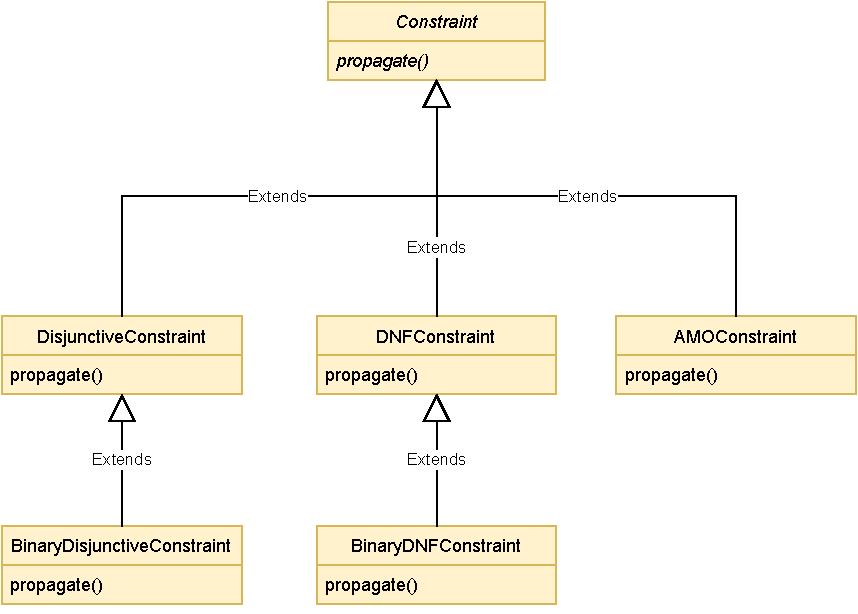
\includegraphics[width=\textwidth]{Classes.pdf}
  \caption{The constraint classes used by the SAT solver}
  \label{fig:constraints}
\end{figure}

Figure \ref{fig:constraints} shows the class diagram of the constraints that are used in the solver. All the constraints in our implementation inherit from the abstract class "Constraint". This superclass allows for a general implementation of the CDCL-algorithm that treats every constraint the same. Of course the propagation of a literal is very different depending on the type of constraint. In order to ensure a correct propagation, every subclass of "Constraint" implements its own "propagate()" method.

\subsection{The "DisjunctiveConstraint" class}

This class contains the implementation of the clause constraints, as the name already suggests. Internally every literal of the clause is kept inside an primitive integer array. Simple arrays have the advantage of minimal memory consumption and very fast access times. The propagate() method makes use of the Two-Watched-Literals algorithm that was already described in chapter \ref{ch:Basics}. That means that there are always two non false literals watched. If any of them turn false, then another non false literal is set as a replacement. If there are no replacement literals left, then the last non false watched literal must be propagated as a unit literal.

\subsection{The "BinaryDisjunctiveConstraint" class}

This is a subclass of the "DisjunctiveConstraint" class. The DisjunctiveConstraint class is already not very computationally expensive, but we considered that an improvement might be possible by dedicating a class to the special case of binary clauses. These binary clauses have the advantage, that if any of the two literals turns false, the other can be instantly propagated. We take advantage of that in the "BinaryDisjunctiveConstraint" class.

\subsection{The "AMOConstraint" class}

This class contains the implementation of the "At-Most-One" constraint. AMO constraints are similar to clauses, because they can be fully described by just a list of literals. Other state of the art SAT solvers normally already encode AMO constraints as clauses in the input file. This allows them to solve these constraints without needing to have an internal representation for the constraint. This goes against what our architecture tries to achieve. We try to leverage the structure of AMO constraints in order to achieve faster solving speeds.
\par
The literals of our AMO constraints are also kept in a primitive integer array similar to the "DisjunctiveConstraint" class. The propagate() method also makes use of watched literals. Contrary to the clauses, every literal in the AMO constraint needs to be watched. This is necessary, because if just a single literal turns true, every other literal needs to be false. So every true literal in an AMO constraint instantly triggers a unit propagation.

\subsection{The "DNFConstraint" class}

This class contains the implementation of the "DNF" constraint. In contrast to the clause and AMO constraints, a DNF constraint can't be simply represented by a list of literals. Internally the class uses an array of primitive integer arrays in order to represent the different terms. Here the minimal memory consumption and fast access speed are the reason, arrays are used. The literal propagation is far more complex in DNF constraints than it is in clauses and AMO constraints. That is the case because a unit propagation needs to start if all non false terms intersect on a literal. This makes it difficult to find an algorithm that is similar to the Two-Watched-Literals algorithm for clauses. The DNFConstraint class therefore uses the algorithm that was already defined in chapter \ref{ch:Analysis}.
\par
Because the algorithm watches all terms of every DNF constraints, we need to make sure that the time that is spent during a visit remains minimal. During the creation of a DNF constraint object, the algorithm therefore pre calculates as list for every literal, that contains all terms that share this literal. These lists can then be efficiently used to check for intersections.

\subsubsection{The "BinaryDNFConstraint" class}

This is a subclass of the DNFConstraint class. During development we recognized that the DNF constraints need a lot of computation time because of the many intersection calculations that need to be done in order to ensure propagation completeness. In the case of binary DNF constraints these calculations are not necessary. That's why the BinaryDNFConstraint class uses simpler techniques. A binary DNF constraint contains only two terms. During the class initialization we check if there are any shared literals between these two terms. These literals need to be unit literals. After that we just watch the two terms of the binary DNF constraint. If one of the terms turns false, the other needs to be instantly propagated. By using this class we can save computational time and memory when the formula has many binary DNF constraints.

There is also the special case of a DNF constraint with only one term. We didn't create a dedicated class for this case, but we considered it in the implementation of the DNFConstraint class. There we check if the constraint has only one term. If that is true, then every literal of this term gets instantly propagated.

\section{The "Formula" class}

This class is the centerpiece of the architecture and contains the whole formula as the name suggests. It is needed to keep track of variable assignments, unit literals, phase saving states, constraints, watched literals and also conflicts.
\paragraph{The "variables" array} is needed in order to keep track of the current variable assignments. It contains an entry for each existing variable. These entries are either "0", "-1" or "1" which mean "no assignment", "false" or "true" respectively.
\paragraph{The "unitLiteralState" array} is similar to the variables array and has an entry for each existing variable. It keeps track if a literal needs to be propagated as a unit literal. The entries are similar to the variables array.
\paragraph{The "phaseSavingLastAssignment" array} also has an entry for each existing variable and keeps track of the last assignment of this variable. This is used to implement the phase saving technique.
\par
An important part of the "Formula" class are the lists that keep track of in which constraint a literal is watched. The "Formula" class contains two arrays for each type of constraint. The first array keeps track of the constraints where the variables are positively watched, and the second array keeps track of the constraints where the variables are negatively watched. Each of these arrays has an entry for each variable. These entries are lists of constraints where the literal is watched.
\par
The most important task of the "Formula" class is the delegation of the literal propagation to the correct constraints. When a literal gets propagated then it selects the correct lists to see where the literal is watched. It then invokes the propagate() method on every constraint that is contained in these lists. During the CDCL-algorithm some learned constraints can be declared obsolete in order to reduce the database size. If such a constraint is encountered then it is removed. If a conflict occurs during the propagation in one of the constraints, then the class also saves the literal and constraint that caused the conflict.

\section{The "SolverAlgorithm" class}

This class contains the implementation of the general solving procedure for the formulas. In an early concept this class was supposed to have several subclasses that each contain different algorithms for SAT solving. Later on this class was re purposed to just hold the general structure of a solving algorithm. This generic algorithm calls several abstract strategy classes that change the course of the algorithm depending on which of their subclasses is used by the dynamic binding of java. Specifically these classes use the strategy pattern for the conflict handling, the restart scheduling and the variable selection.

\begin{algorithm}
\caption{solve(formula)}\label{alg:cap}
\begin{algorithmic}
\State $trail \gets \{\}$
\While{$trail.size() \neq formula.numberOfVariables()$}
	\State $unitPropagation()$
\If{$formula.hasConflict()$}
	\State $conflictHandlingStrategy()$
	\State $restartHandlingStrategy()$
\Else
    \State $x \gets variableSelectionStrategy()$
    \State $formula.propagate(x)$
    \State $trail.assign(x)$
\EndIf
\EndWhile
\end{algorithmic}
\end{algorithm}

\section{The "ConflictHandlingStrategy" class}

\begin{figure}[htbp]
  \centering
  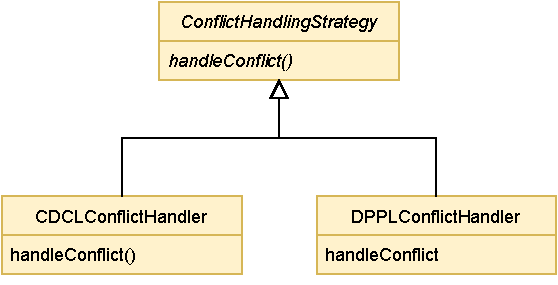
\includegraphics[scale=1.2]{ConflictHandlingStrategy.pdf}	
  \caption{The conflict handling strategies used by the solver}
  \label{fig:conflictHandling}
\end{figure}

Figure \ref{fig:conflictHandling} shows the ConflictHandlingStrategy class and its two subclasses. The two subclasses both have a different approaches to handling the conflicts that occur during the solving process. There is the "DPLLConflictHandler" that uses the conflict handling strategy of the DPLL algorithm in order to resolve conflict. And there is the "CDCLConflictHandler" that uses Conflict-Driven-Clause-Learning in order to resolve the conflicts
\par
The DPLLConflictHandler uses a simple procedure independent of which type of conflict occurs during the solving process. If a conflict occurs in the algorithm then this class unassigns every variable on the trail until it finds a variable that wasn't assigned by unit propagation and hasn't been assigned both "true" and "false" as values. This variable then gets propagated with the value that hasn't been tried yet. This procedure gets repeated until every combination of variable assignments have been tried.
\par
The CDCLConflictHandler makes use of our modified version of the CDCL-algorithm. If a conflict occurs between two clauses then the algorithm just follows the normal procedure of the already described CDCL-algorithm. If a conflict occurs between two other constraints, then the class determines the constraint that the conflict occurred in and calls its "handleConflict()" method. This call gives the conflict constraint the responsibility on how to handle the conflict.

\subsection{The conflict handling}

Each constraint type has an implementation of the "handleConflict()" method. This method always gets called on the constraint in which the conflict occurred in. In this method the constraint determines the constraint that is the reason for this conflict. The "Formula" class keeps track of which constraint caused the propagation of a unit literal. We call these constraints the "reason constraint" of the unit literal. The conflict constraint therefore determines the reason constraint of the conflict literal. Now depending on which type of constraints are involved in the conflict, we apply the conflict resolution rules that were determined in chapter \ref{ch:Analysis} and derive the learnable constraints.

\subsection{The backtracking process}

After the learn able constraints are determined the CDCLConflictHandler first checks if the set of learned constraints is either empty or contains a constraint that is empty. In this case the formula is unsatisfiable and the algorithm stops
\par
In order for the learned constraint to have an effect, the algorithm needs to backtrack the trail enough so that each learned constraint is at least still satisfiable. The necessary decision level to ensure this condition is the minimum decision level over all needed decision levels of all learned constraints. Each constraint type has a "getNeededDecisionLevel()" method that determines the necessary level depending on the constraint type. The algorithm backtracks to the determined decision level by unassigning all variables on the trail until the needed level is reached.

\subsection{Constraint database reduction}

The standard CDCL-algorithm and our derived version have in common that a long solving process results in a large amount of constraints that are learned. The constraint database will reach a point where the advantage of the learned constraints is overshadowed by the overhead of memory and propagation time that is needed to visit them. Therefore we implemented a constraint database reduction algorithm that gets less aggressive the more reductions occur. If the number of conflicts reaches 20000 then the database gets halved. With every database reduction this threshold gets elevated by 500. Before halving the database we sort it according to the LBD scores of the learned constraints.

\section{The "RestartSchedulingStrategy" class}

\begin{figure}[htbp]
  \centering
  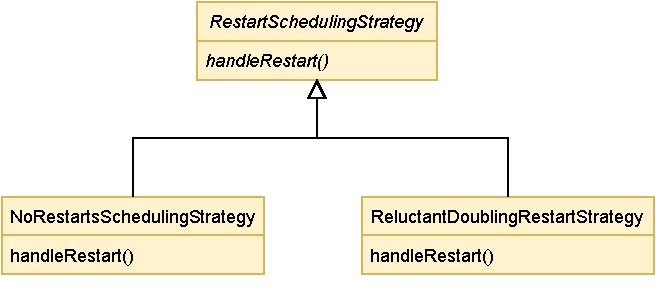
\includegraphics[scale=1.2]{RestartSchedulingStrategy.pdf}	
  \caption{The restart strategies used by the solver}
  \label{fig:restartScheduling}
\end{figure}


Figure \ref{fig:restartScheduling} shows the RestartSchedulingStrategy class and its two subclasses. The two subclasses of contain different implementations on how to handle restarts during the solving process. The "NoRestartsSchedulingStrategy" class is a simple stub class that just never restarts the solving process. This is necessary if the user doesn't want any restarts. The "ReluctantDoublingRestartStrategy" class makes use of the static restarting algorithm based on the Luby sequence. In order to ensure an efficient implementation, it uses the reluctant doubling algorithm in order to calculate the sequence.

\section{The "VariableSelectionStrategy" class}

\begin{figure}[htbp]
  \centering
  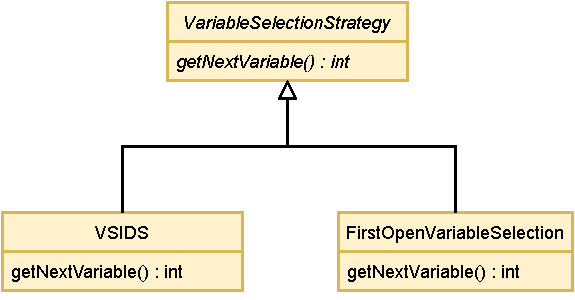
\includegraphics[scale=1.2]{VariableSelectionStrategy.pdf}
  \caption{The different variable selection strategies used by the solver}
  \label{fig:variableSelection}
\end{figure}

Figure \ref{fig:variableSelection} shows the abstract class "VariableSelectionStrategy" and its two subclasses. The subclasses contain different implementations of decision heuristics that determine the next variable that gets assigned.

The "FirstOpenVariableSelection" class contains a very simple implementation. It just iterates over the variables array of the "Formula" class and determines the next variable by just choosing the first variable that currently has no assignment.

The "VSIDS" class contains the implementation of the exponential VSIDS (EVSIDS) decision heuristic. In order to use this heuristic, the "Formula" class keeps an array of variable occurrences. This array has an entry for each variable in the formula, that contains the number of occurrences. Later on this occurrence count will be adjusted and used as a general score. During a conflict we keep track of which variables are involved. After that the score of these variables gets adjusted by using the following formula:
\begin{displaymath}
score = score + {1.01}^{conflictCounter}
\end{displaymath}
In the "VSIDS" class we keep a priority queue of every variable, sorted by their score. If the next variable needs to be selected, the priority queue gets polled until we draw a variable that is currently unassigned. This variable is then chosen as the next variable that gets propagated. During the backtracking process after a conflict, we fill the priority queue with every variable that gets unassigned.

\section{The "IncrementalCDCLSolver" class}

\begin{figure}[htbp]
  \centering
  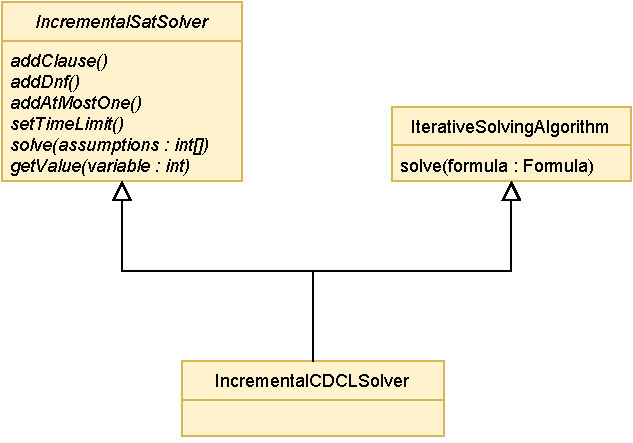
\includegraphics[scale=1.2]{IncrementalSatSolver.pdf}
  \caption{The incremental SAT solver interface and its subclass}
  \label{fig:incrementalSAT}
\end{figure}

Figure \ref{fig:incrementalSAT} shows the IncrementalCDCLSolver class. The class inherits from the "IterativeSolvingAlgorithm" class, so that it can make use of the already implemented "solve()" method. It then also implements the "IncrementalSatSolver" interface which offers the methods to add clauses, AMO constraints and DNF constraints directly in the code instead of having to work with the "*.cnf" files on the hard drives. This is especially useful while doing experiments that constantly change the number of variables or the amount of constraints.
